\documentclass[11pt, a4paper]{article}

% --- PACKAGES ---
\usepackage[utf8]{inputenc}
\usepackage[T1]{fontenc}
\usepackage{geometry}
\usepackage{graphicx}
\usepackage{listings}
\usepackage{hyperref}
\usepackage{amsmath}
\usepackage{amsfonts}
\usepackage{amssymb}
\usepackage{times}
\usepackage{xcolor}

% --- GEOMETRY ---
\geometry{a4paper, margin=1in}

% --- HYPERREF SETUP ---
\hypersetup{
    colorlinks=true,
    linkcolor=blue,
    filecolor=magenta,      
    urlcolor=cyan,
}

% --- LISTINGS (CODE) SETUP ---
\lstdefinelanguage{text}{}
\lstset{
    language=SQL,
    basicstyle=\ttfamily\small,
    keywordstyle=\color{blue},
    stringstyle=\color{red},
    commentstyle=\color{green!60!black},
    showstringspaces=false,
    breaklines=true,
    frame=single,
    numbers=left,
    numberstyle=\tiny\color{gray},
    captionpos=b
}

% --- DOCUMENT INFO ---
\title{Design and Implementation of a Scalable Multi-User Database System for Smart Healthcare Management}
\author{Serhet Gökdemir \\ 21058024}
\date{2026}

% --- DOCUMENT START ---
\begin{document}

% Avoid duplicate page anchors by not reusing page numbers in the PDF
\hypersetup{pageanchor=false}
\pagenumbering{gobble}

\maketitle
\thispagestyle{empty}

\newpage
\tableofcontents
\thispagestyle{empty}

\newpage
\pagenumbering{arabic}
\hypersetup{pageanchor=true}

% --- SECTIONS ---
\section{Requirements Analysis}

\subsection{Introduction}
This section outlines the requirements for the Smart Healthcare Management database system. The primary objective is to create a robust, scalable, and secure system that supports multiple user roles and complex medical data interactions.

\subsection{User Roles and Permissions}
The system will support the following user roles:
\begin{itemize}
    \item \textbf{Patient:} Can view their personal information, appointments, prescriptions, and lab results.
    \item \textbf{Doctor:} Can manage patient records, schedule appointments, issue prescriptions, and order lab tests.
    \item \textbf{Administrator:} Can manage hospital, department, and doctor information, overseeing the system's structural data.
\end{itemize}

\subsection{Core Entities}
The main entities identified for the system are:
\begin{itemize}
    \item Patient
    \item Doctor
    \item Hospital
    \item Department
    \item Appointment
    \item Prescription
    \item Lab Result
    \item Insurance
    \item Bill
\end{itemize}

\subsection{Core Relationships}
Key relationships between entities include:
\begin{itemize}
    \item A \textbf{Doctor} can have many \textbf{Patients} (1-to-N).
    \item A \textbf{Patient} can have many \textbf{Appointments} (1-to-N).
    \item A \textbf{Hospital} has many \textbf{Departments} (1-to-N), and each \textbf{Doctor} belongs to one \textbf{Department} (N-to-1).
    \item A \textbf{Doctor} can have multiple \textbf{Specialties} (N-to-M), implemented via a linking table.
    \item An \textbf{Appointment} must be associated with exactly one \textbf{Patient} and one \textbf{Doctor}.
\end{itemize}

\subsection{Constraints and Business Rules}
The system must enforce the following rules:
\begin{itemize}
    \item A prescription can only be written by an authorized doctor.
    \item Every appointment must be linked to an existing patient and doctor.
    \item Patient medical records are confidential and can only be accessed by authorized personnel.
\end{itemize}

\section{ER and EER Models}

\subsection{ER Diagram}
The Entity-Relationship (ER) diagram provides a high-level view of the database structure, including entities, their attributes, and the relationships between them.

\begin{figure}[h!]
    \centering
    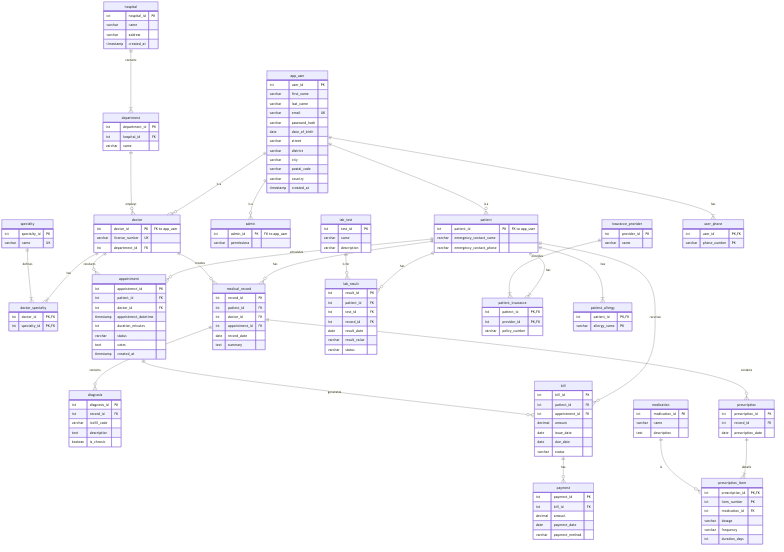
\includegraphics[width=\textwidth]{../er_diagram.png}
    \caption{Entity-Relationship (ER) Diagram.}
    \label{fig:er_diagram}
\end{figure}

\textit{Note: You need to export your Mermaid 'er\_diagram.mmd' as a PNG file and place it in the parent project folder.}

\subsection{Enhanced ER (EER) Diagram}
The Enhanced ER (EER) diagram extends the ER model with concepts like specialization and generalization. In our model, an \texttt{app\_user} supertype is specialized into \texttt{patient}, \texttt{doctor}, and \texttt{admin} subtypes.

\begin{figure}[h!]
    \centering
    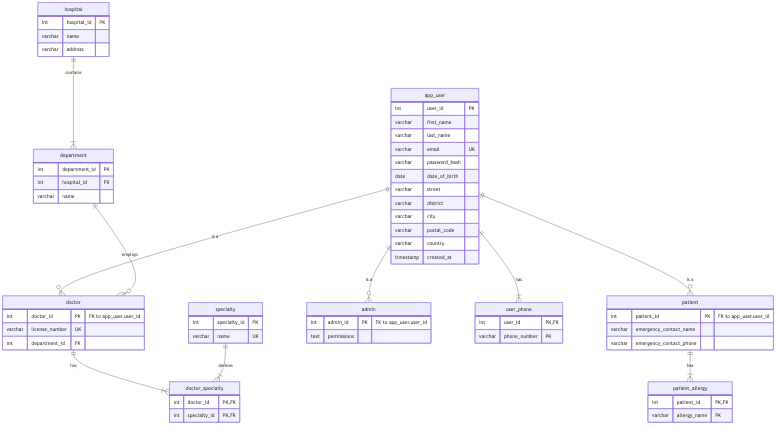
\includegraphics[width=\textwidth]{../eer_diagram.png}
    \caption{Enhanced Entity-Relationship (EER) Diagram.}
    \label{fig:eer_diagram}
\end{figure}

\textit{Note: You need to export your Mermaid 'eer\_diagram.mmd' as a PNG file and place it in the parent project folder.}

\subsubsection{Explanation of EER Concepts}
Here, we used specialization to model different types of users. For example, \texttt{doctor} and \texttt{patient} are specializations of a more general \texttt{app\_user} entity, inheriting common attributes like name and contact information while also having their own specific attributes.

\section{Mapping to Relational Model}
The ER/EER model was mapped to a relational schema. This section presents the final table structures, including primary keys, foreign keys, and other constraints.

\subsection{Relational Schema}
The following SQL script contains the \texttt{CREATE TABLE} statements for all tables in the database.

\lstinputlisting[language=SQL, caption={Relational Schema (\texttt{schema.sql})}]{../schema.sql}

\subsection{Mapping Rules Applied}
Key mapping decisions included:
\begin{itemize}
    \item \textbf{N:M Relationships:} Many-to-many relationships, such as `Doctor\_Department`, were implemented using a separate linking table.
    \item \textbf{Weak Entities:} Weak entities like `Prescription` are identified by a foreign key from their owner entity (`Patient` or `Appointment`).
    \item \textbf{Multivalued Attributes:} If any existed, they would be handled by creating a separate table.
\end{itemize}

\section{Functional Dependencies and Normalization}

\subsection{Functional Dependencies (FDs)}
This section lists the functional dependencies identified for the major tables in the schema.

\begin{verbatim}
-- Copy the content from your fd.md file here.
-- Example:
-- For the Patient table:
-- PatientID -> FirstName, LastName, BirthDate, PhoneNumber

-- For the Doctor table:
-- DoctorID -> FirstName, LastName, Specialty
\end{verbatim}
\textit{Note: Please copy the content from your `fd.md` file and paste it into the verbatim block above.}

\subsection{Normalization Steps}
The schema was normalized to BCNF to reduce data redundancy and improve data integrity. The process is described below.

\begin{verbatim}
-- Copy the content from your normalization.md file here.
-- Describe the steps taken to achieve 1NF, 2NF, 3NF, and BCNF.
-- Show "before" and "after" table structures for each step.
\end{verbatim}
\textit{Note: Please copy the content from your `normalization.md` file and paste it into the verbatim block above.}

\section{SQL Implementation and Advanced Queries}

\subsection{Data Insertion}
The database was populated with sample data to simulate a real-world environment. The script below shows a few example \texttt{INSERT} statements.

\lstinputlisting[language=SQL, caption={Sample Data Insertion (\texttt{data.sql})}, firstline=1, lastline=15]{../data.sql}

\subsection{Advanced SQL Queries}
At least 10 complex queries were developed to test the database's capabilities for retrieving meaningful information. These queries include joins, aggregations, and subqueries.

\lstinputlisting[language=SQL, caption={Advanced Queries (\texttt{queries.sql})}]{../queries.sql}

\subsubsection{Query Outputs}
\textit{Optional: You can run the queries and paste selected outputs here (e.g., inside a \texttt{verbatim} environment or as a formatted table). Outputs are not required to understand the schema and query design.}

\textbf{Query 1: List scheduled appointments with patient/doctor/hospital/department.}
\begin{verbatim}
-- (Optional output)
\end{verbatim}

\textbf{Query 3: List patients with no appointments.}
\begin{verbatim}
-- (Optional output)
\end{verbatim}

\section{Relational Algebra \& Calculus}
This section provides 5 queries written in both Relational Algebra and Tuple Relational Calculus, corresponding to some of the advanced SQL queries.

\begin{verbatim}
-- Copy the content from your relational_algebra_and_calculus.md file here.
-- Example:

-- Query 1: Find all patients born after 2000.

-- Relational Algebra:
-- \sigma_{BirthDate > '2000-01-01'}(Patient)

-- Tuple Relational Calculus:
-- {t | t \in Patient \wedge t.BirthDate > '2000-01-01'}
\end{verbatim}
\textit{Note: Please copy the content from your \texttt{relational\_algebra\_and\_calculus.md} file and paste it into the verbatim block above.}

\section{Indexing and File Structures}

\subsection{Index Implementation}
To optimize query performance, several indexes were created. The choices include B+ Tree indexes for range queries and Hash indexes for exact lookups where applicable.

\lstinputlisting[language=SQL, caption={Index Creation (\texttt{sql/indexing.sql})}]{../sql/indexing.sql}

\subsection{Performance Analysis}
This section discusses the performance impact of the implemented indexes.

\subsubsection{Indexed vs. Non-Indexed Query Performance}
We compared the execution time of several key queries before and after creating indexes. For example, finding all appointments for a specific patient, retrieving a doctor's appointments within a date range, or listing a patient's lab history sorted by date.

\textbf{Example Query: Find all appointments for a specific patient.}
\begin{itemize}
    \item \textbf{Without Index:} The database may perform a sequential scan on the \texttt{appointment} table. See the \texttt{EXPLAIN ANALYZE} output for the plan and timing.
    \item \textbf{With B+ Tree Index on \texttt{appointment(patient\_id)}:} The database can use an index scan to quickly locate matching rows. See the \texttt{EXPLAIN ANALYZE} output for the plan and timing.
\end{itemize}

On larger datasets, indexes are expected to improve query performance by reducing the amount of data scanned and by avoiding expensive sorts. With a small sample dataset, PostgreSQL may still choose sequential scans, which is not an error but a cost-based planner decision.


\end{document}
